\documentclass{beamer}
\usetheme{metropolis}           % Use metropolis theme
%\usepackage[german]{babel}  
\usepackage[utf8]{inputenc}	%dt Sonderzeichen wie ß
\usepackage{tikz}
\usepackage{amssymb}
\usepackage{multirow}
\usepackage{pgfpages}
\usepackage{cite}
\usepackage{graphicx}
\usepackage{animate}


\usepackage{multimedia}
\usepackage{float}
\usepackage{subfig}
\usepackage{svg}
\usepackage{enumitem}


%\setbeameroption{show notes on second screen=right}  %% Uncomment this to get Notes


%\renewcommand*{\figurename}{Abb.}




\title{Speechrecognition}
\date{9.11.2018}
\author{Robert Feldhans}
\institute{Seminar Robocup}
\begin{document}
	\maketitle
	
	\begin{frame}{Motivation}
		Why even bother?
		\begin{itemize}
			\item[-] faster and more general way to give robots commands
			\item[-] a necessity for casual users
			\item[-] user does not need additional hardware
		\end{itemize}
	\end{frame}
	
	\begin{frame}{Content}
		
		\begin{alertblock}{What is Speechrec? What does it consist of?}
		\end{alertblock}
		
	\end{frame}
	
	\begin{frame}{Content}
		\setbeamertemplate{section in toc}[sections numbered]
		\tableofcontents[hideallsubsections]
	\end{frame}
	
	\begin{frame}{Quick example}
		content...
	\end{frame}
	
	
	\section{Hardware}%%%%%%%%%%%%%%%%%%%%%%%%%%%%%%%%%%%%%%%%%%%%%%%%%%%%%%%%%%%%%%%%%%%%%%%%%%%%%%%%%%%%%%%%
	
	\begin{frame}{Microphones}
		\begin{figure}[ht]
			\centering
			\subfloat[dynamic microphone]{
				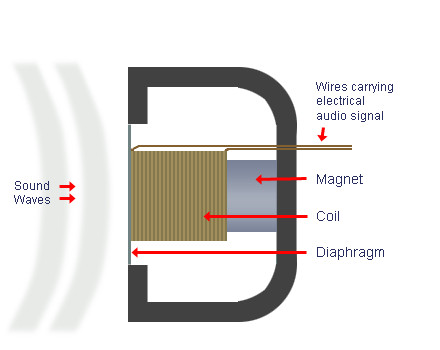
\includegraphics[width=.5\textwidth]{Bilder/mic-dynamic.jpg}
			}
			\subfloat[condenser microphone]{
				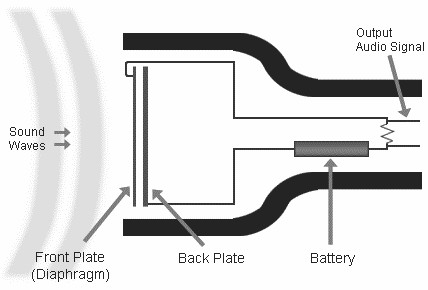
\includegraphics[width=.5\textwidth]{Bilder/Condenser-Mic-Diagram.jpg}
			}
			\caption{Different kinds of microphones. Source: http://www.onlinetuner.co}
		\end{figure}
	\end{frame}
	
	\begin{frame}{Audio}
		Microphones provide audio defined by:
		\begin{itemize}[leftmargin=*,labelindent=50pt]
			\item[rate:] resolution in time domain
			\item[bitrate:] resolution in quality domain
			\item[endian:] representation of signal
			\item[channel:] amount of channels 
			\item[interleaving:] representation of signal by channel
		\end{itemize}
	\end{frame}
	
	\begin{frame}{Microphones: Polar Patterns}
		\begin{figure}[ht]
			\centering
			\subfloat[cardioid pattern]{
				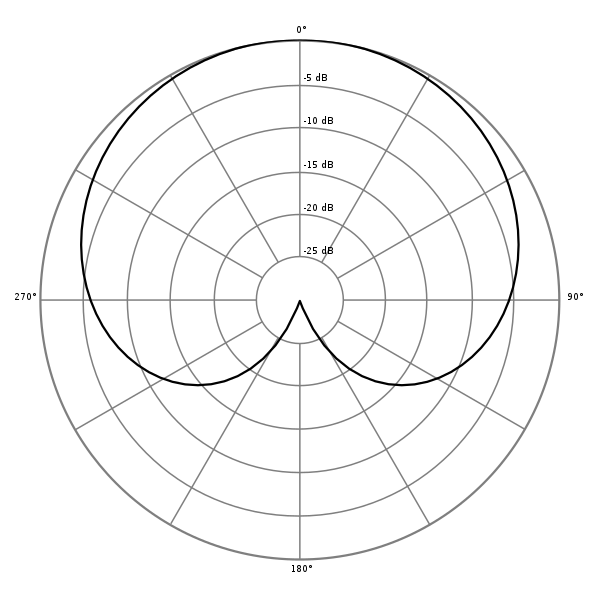
\includegraphics[width=.33\textwidth]{Bilder/Polar_pattern_cardioid.png}
			}
			\subfloat[directional pattern]{
				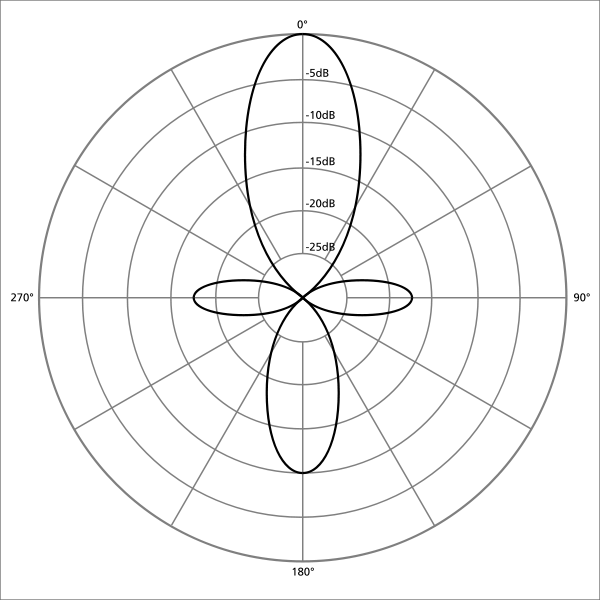
\includegraphics[width=.33\textwidth]{Bilder/Polar_pattern_directional.png}
			}
			\subfloat[omnidirectional pattern]{
				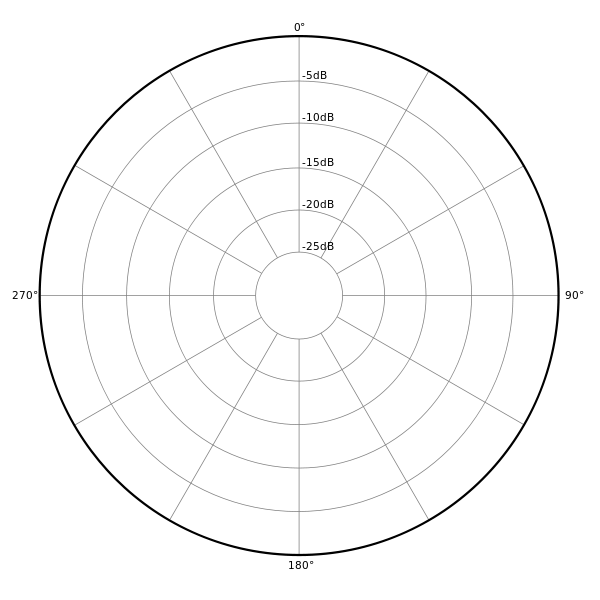
\includegraphics[width=.33\textwidth]{Bilder/Polar_pattern_omnidirectional.png}
			}
			\caption{Diffrent kinds of microphone pattern. Source: Wikipedia}
		\end{figure}
	\end{frame}
	
	\begin{frame}{Microphone Arrays}
		\begin{alertblock}{Why?}
			\begin{itemize}
				\item[-] more sensors are always better
				\item[-] several microphones can be linked together to reduce noise
				\item[-] by analysing the distribution of signals and frequencies in time we can even detect the direction from where a sound was emitted
			\end{itemize}
		\end{alertblock}
	\end{frame}
	
	\begin{frame}{Microphone Arrays II}
		\begin{figure}[ht]
			\centering
			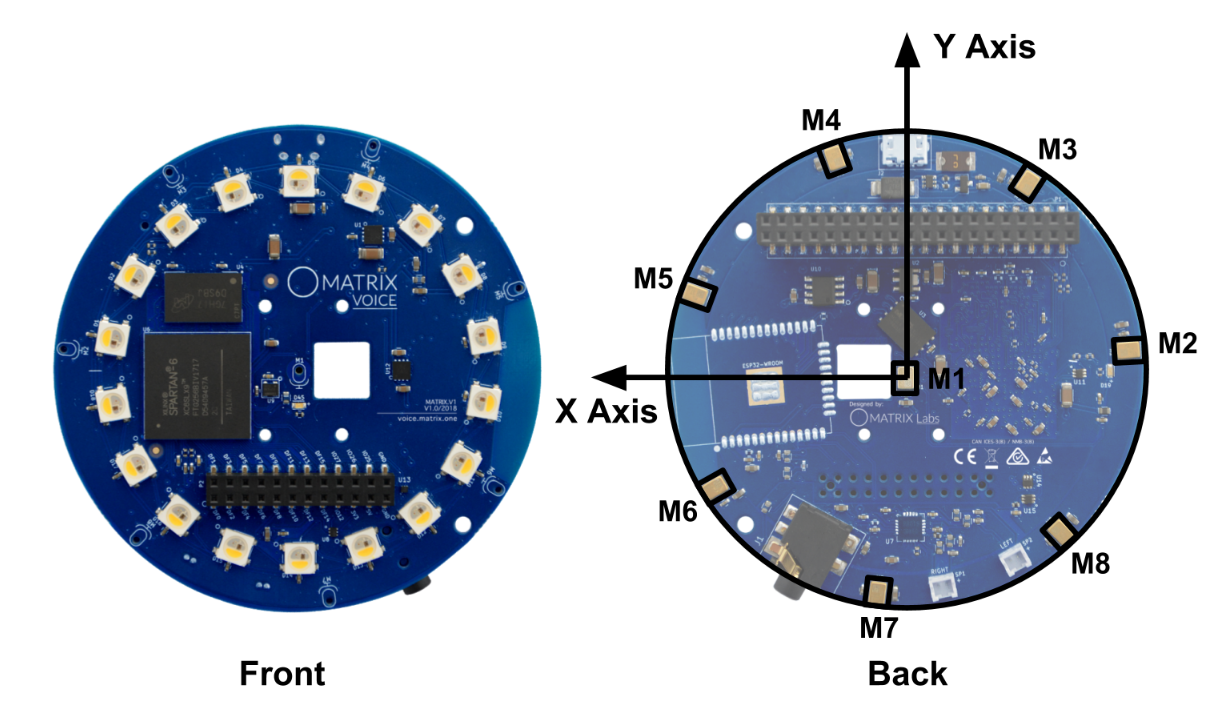
\includegraphics[width=.8\linewidth]{Bilder/mic_voice_position.png}
			\caption{Matrix Voice, a microphone array. Source: https://matrix-io.github.io/matrix-documentation/matrix-voice/resources/microphone/}
		\end{figure}
	\end{frame}
	
	\begin{frame}{What do we use?}
		Tobi:
		\pause
		One or two directional microphones, 2 additional for sound source localization.
		
		Pepper:
		\pause
		An array of four omnidirectional microphones inside of the head.
		
		Tiago:
		\pause
		Stereo microphones in the torso (black spots under his head).
	\end{frame}
	
	\begin{frame}{Alsa}
		The Advanced Linux Sound Architecture manages all your physical and virtual microphones and speakers.
		\begin{itemize}
			\item[-] It controls volume and gain
			\item[-] It controls rate and bitrate of captured audio, as well as other properties
			\item[-] Extensive configuration makes basically any imaginable microphone constellation possible
		\end{itemize}
		
		\pause
		
		Honorable mention: pulseaudio
		\pause
		\begin{itemize}
			\item[-] \emph{many} extensions (called modules) to suit all kinds of needs
			\item[-] eg. virtual devices over network, on the fly filtering, etc.
		\end{itemize}
	\end{frame}
	
	\section{Localisation}%%%%%%%%%%%%%%%%%%%%%%%%%%%%%%%%%%%%%%%%%%%%%%%%%%%%%%%%%%%%%%%%%%%%%%%%%%%%%%%%%%%%%%%%
	
	\begin{frame}{Sound Source Localisation}
		Basic Idea:
		\begin{itemize}
			\item[-] more than one microphone is required
			\item[-] four microphones are required for "exact" localisation
			\item[-] can be seperated into 2 sub-problems: time delay estimation and position estimation
			\item[-] time delay estimation guesses the time differences with which a sound arrives at different microphones
			\item[-] position estimation  tries to locate the soundsource based on these guesses
		\end{itemize}
	\end{frame}
	
	\begin{frame}{Time Delay Estimation}
		Approaches:
		\begin{itemize}[leftmargin=*,labelindent=16pt]
			\item[-] time domain approximation
			\item[-] frequency based
			\item[-] statistical approaches
		\end{itemize}
		
		\begin{figure}[ht]
			\centering
			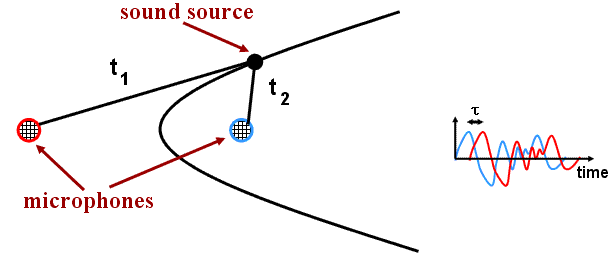
\includegraphics[width=.8\linewidth]{Bilder/ssl.png}
			\caption{Source: https://cecas.clemson.edu/~stb/research/acousticloc/}
		\end{figure}
	\end{frame}
	
	\begin{frame}{Position estimation}
		Sound source localisation is not exact
		\begin{itemize}
			\item[-] TDE is just an estimation (duh)
			\item[-] because of superposition TDE may provide false positives
			\item[-] position estimation can be interpreted as (n-1)-dimensional optimization problem
			\item[-] optimization problems can be solved by eg. gradient descent or conjugate gradients
		\end{itemize}
		(see Mario Botsch's Scientific Computing course for more information about solving these problems)
	\end{frame}
	
	\section{Signal Enhancing}%%%%%%%%%%%%%%%%%%%%%%%%%%%%%%%%%%%%%%%%%%%%%%%%%%%%%%%%%%%%%%%%%%%%%%%%%%%%%%%%%%%%%%%%
	
	\begin{frame}{Beamforming}
		content...
	\end{frame}
	
	\section{Voice Activation Detection}%%%%%%%%%%%%%%%%%%%%%%%%%%%%%%%%%%%%%%%%%%%%%%%%%%%%%%%%%%%%%%%%%%%%%%%%%%%%%%%%%%%%%%%% rather done
	
	\begin{frame}{What we use}
		\begin{figure}[ht]
			\centering
			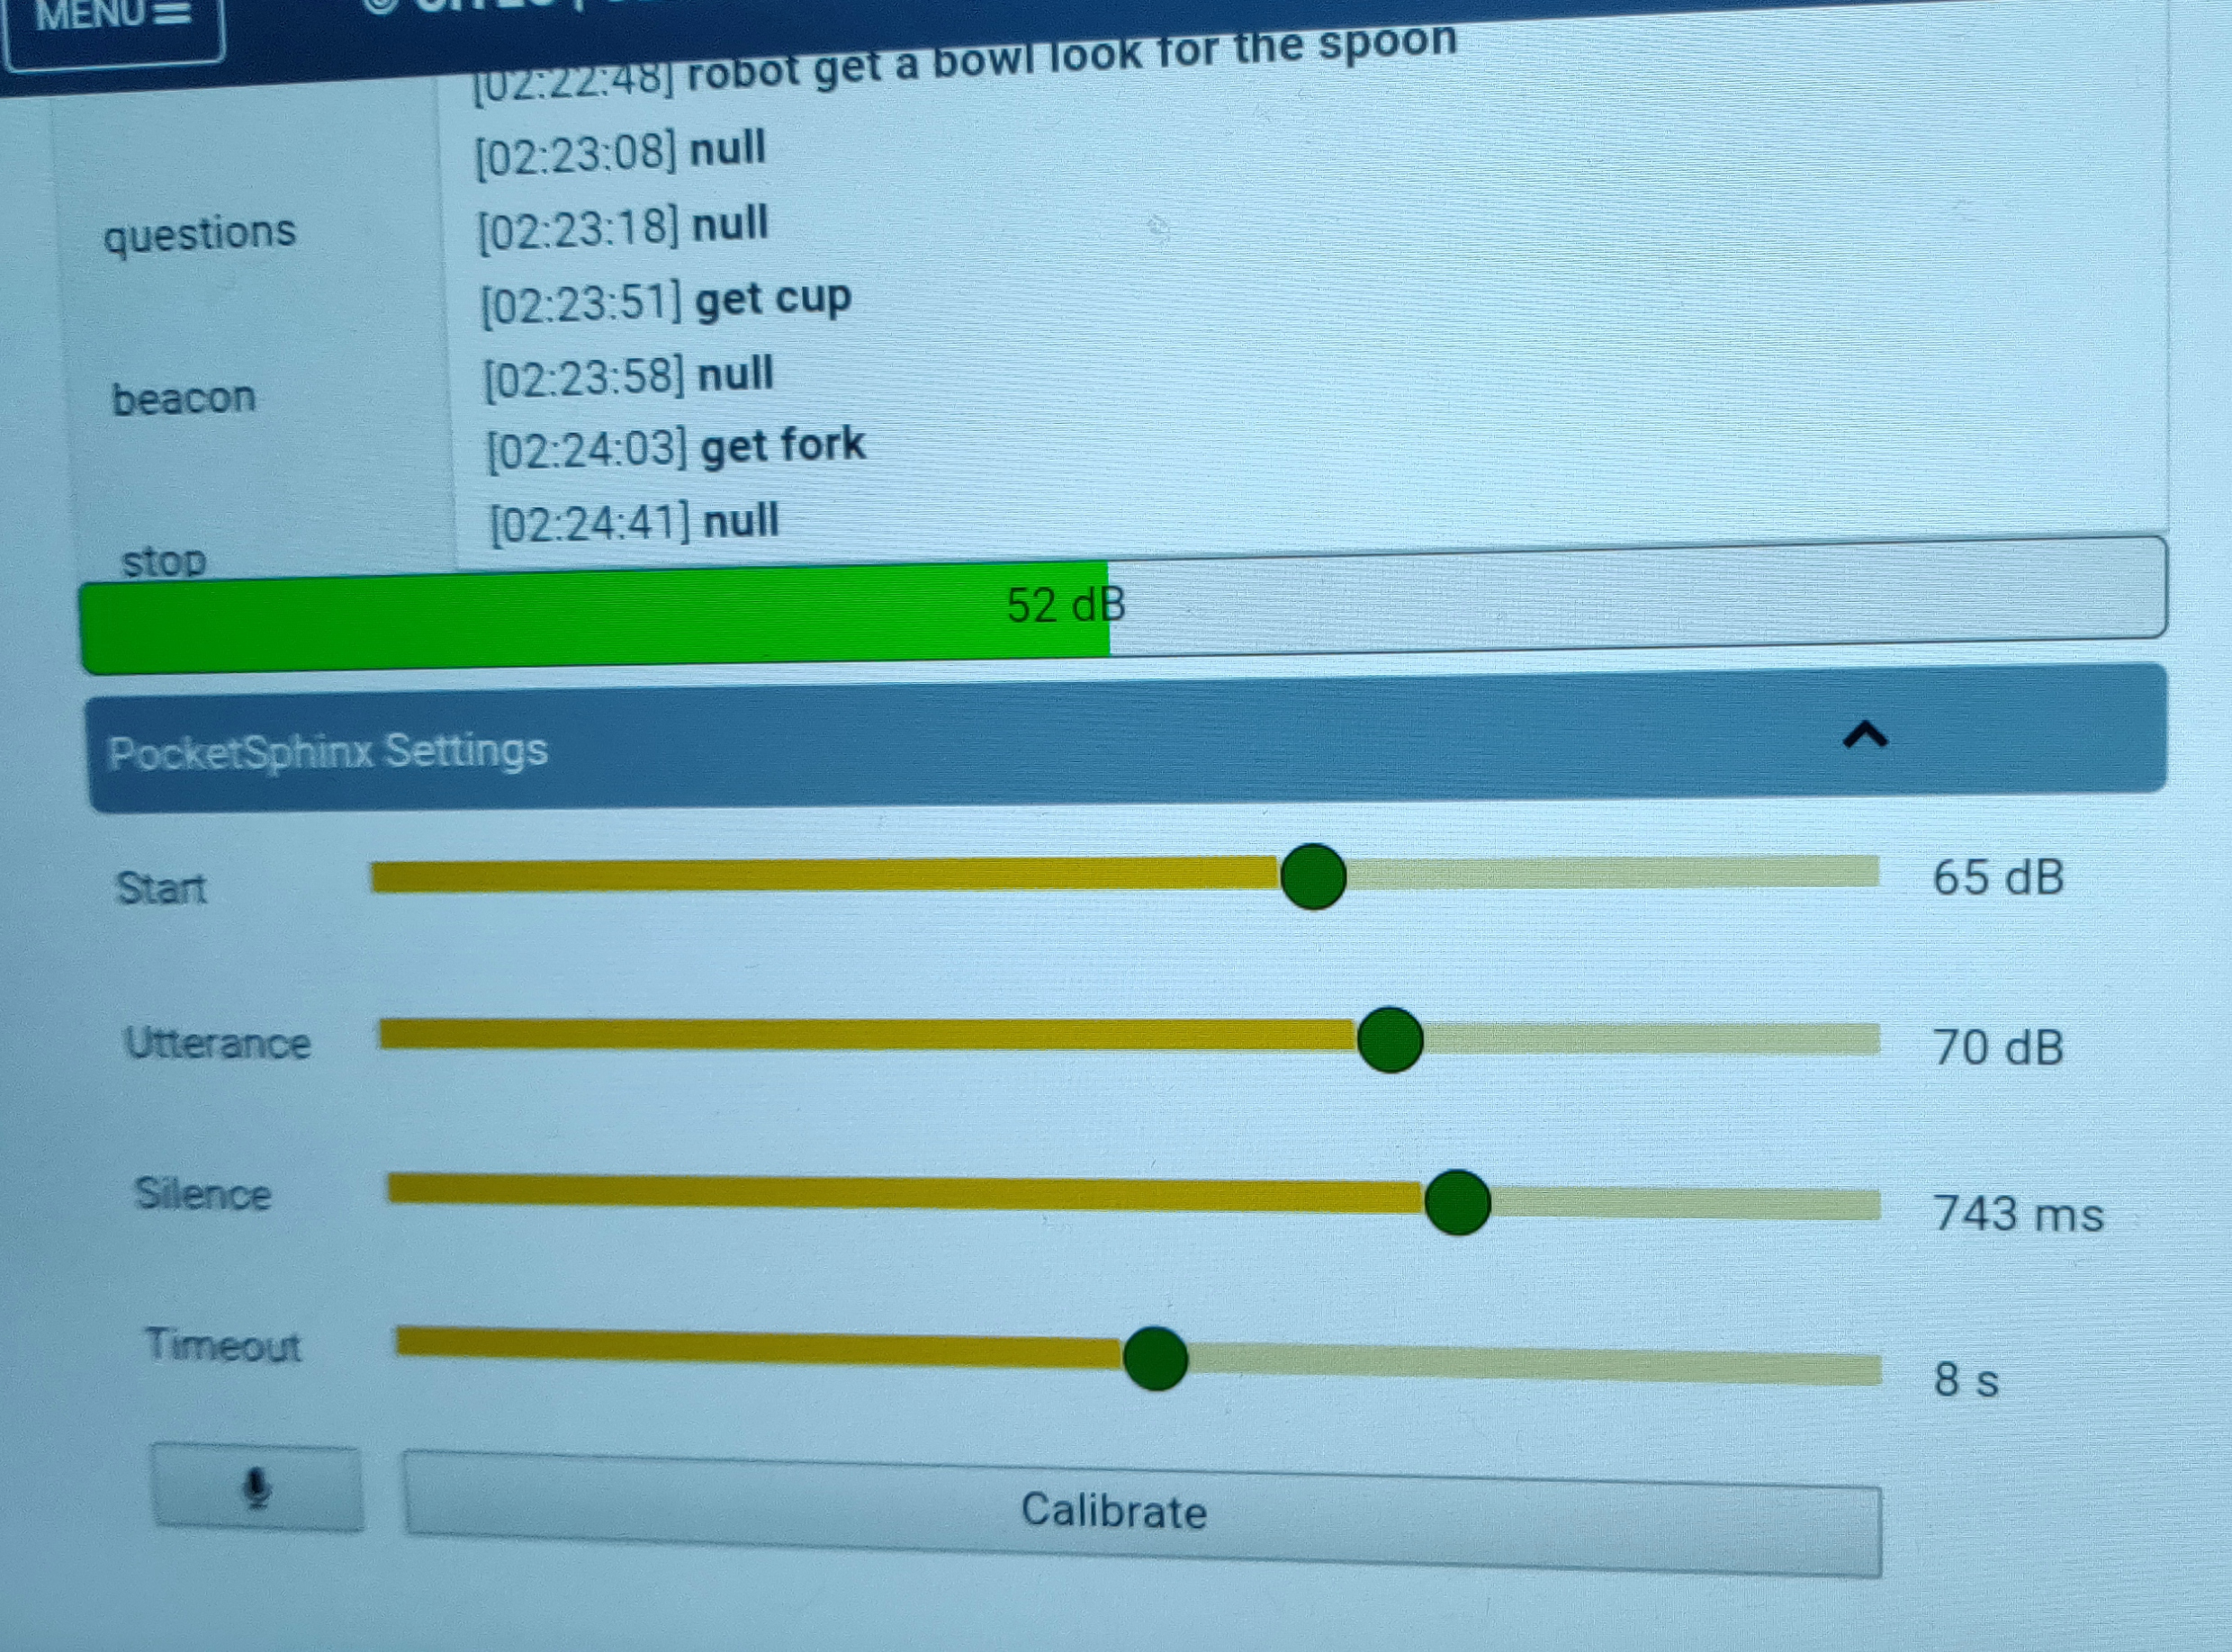
\includegraphics[width=.8\linewidth]{Bilder/VAD.jpg}
			\caption{Double threshold voice activation detection}
		\end{figure}
	\end{frame}
	
	\begin{frame}{What we use II}
		A voice activation detection based on audio loudness with three states: 
		\begin{itemize}[leftmargin=*,labelindent=32pt]
			\item[idle] Start in this state
			\item[starting] switch to this state if the audio $>$ StartDb and stay here as long as audio $>$ UtteranceDb
			\item[ending] switch to this state if the audio $<$ UtteranceDb and stay as long as specified via Silence, then return to idle
		\end{itemize}
		A maximum audio length can be specified via Timeout
	\end{frame}
	
	\begin{frame}{Other approaches}
		Based on...
		\begin{itemize}[leftmargin=*,labelindent=32pt]
			\item[loudness] based on decibel calculation, it will only take into account the single most extreme value in an audio frame
			\item[energy] in contrast to loudness-based approaches, energy calculation will take all values in an audio frame into consideration
			\item[frequency] will calculate frequencies and search for those typically used by human speech
		\end{itemize}
	\end{frame}
	
	\section{Speaker Recognition}%%%%%%%%%%%%%%%%%%%%%%%%%%%%%%%%%%%%%%%%%%%%%%%%%%%%%%%%%%%%%%%%%%%%%%%%%%%%%%%%%%%%%%%%
	
	\section{Speech Recognition}%%%%%%%%%%%%%%%%%%%%%%%%%%%%%%%%%%%%%%%%%%%%%%%%%%%%%%%%%%%%%%%%%%%%%%%%%%%%%%%%%%%%%%%%
	
	\begin{frame}{Approaches}
		There are three big approaches for consumer/ robotics speech recognition:
		\begin{itemize}
			\item Hidden Markov Models
			\item Deep Learing
			\item Online Services
		\end{itemize}
	\end{frame}
	
	\begin{frame}{Hidden Markov Models}
		Hidden Markov models are statistical models where a system is assumed to be a markov process with hidden states.
		\begin{itemize}
			\item[-] imagine a statemachine where the transitions are modeled by probabilities
			\item[-] states in this statemachine can be roughly understood as phonemes
			\item[-] a most probable path through the model can be computed for a given sequence of signals or data 
			\item[-] this path is can then be mapped to a spoken word or sequence of words
			\item[-] states are unknown (hidden) and assumed via probabilities
		\end{itemize}
	\end{frame}
	
	\begin{frame}{Sphinx}
		A HMM based group of application which use 
		\begin{itemize}
			\item[-] a speech model (models phenomes)
			\item[-] a dictionary (maps phonemes to words)
			\item[-] a language model (probabilities of word sequences)
		\end{itemize}
		
		Recent versions can provide quasi-free speech recognition.
	\end{frame}
	
	\begin{frame}{Deep Learning \& DeepSpeech}
		Deep Learning
		\begin{itemize}
			\item[-] \emph{very} big field
			\item[-] computationally expensive concept to abstract high level information out of big chunks of data
		\end{itemize}
		\pause
		DeepSpeech
		\begin{itemize}
			\item[-] ML architecture by Baidu
			\item[-] several implementations, e.g. by mozilla using tensorflow
			\item[-] detects free speech, but is somewhat phoneme based
			\item[-] currently one of the best architectures in regards to word error rate
		\end{itemize}
	\end{frame}
	
	\begin{frame}{Google/Bing/... Online Speechrec}
		Commercial "Cloud" services provided by companies like Google, Amazon, Microsoft, etc.
		\begin{itemize}
			\item[-] kind of a blackbox
			\item[-] need \emph{fast} internet connections
			\item[-] typically better results than local speechrec
			\item[-] not free, can be quite expensive if used extensively
		\end{itemize}
	\end{frame}
	
	
	\begin{frame}{Grammar vs Grammarless/Freespeech}
		Grammar based recognition
		\begin{itemize}
			\item[-] by restraining accepted inputs the results can be more precise
			\item[-] mapping result to action can be very easy
			\item[-] must be supported by approach \emph{and} implementation
			\item[-] best suited for controlled environments/ use cases
		\end{itemize}
		Freespeech
		\begin{itemize}
			\item[-] usually seen in deep learning approaches
			\item[-] any spoken word can be detected
			\item[-] go-to apporach for extremely complex use cases
		\end{itemize}
	\end{frame}
	
	\begin{frame}{Corrected Spelling vs Phoneme based recognition}
		Corrected spelling
		\begin{itemize}
			\item[-] needs a dictionary
			\item[-] guarantees correct spelling (important for further processing)
			\item[-] makes a very robust speech recognition (esp. in combination with grammars)
		\end{itemize}
		Phoneme bases recognition
		\begin{itemize}
			\item[-] does not need any kind of dictionary
			\item[-] adapts better to new/unique words
			\item[-] usually embraced by deep learning approaches
		\end{itemize}
	\end{frame}
	
	\begin{frame}{What do we use?}
		For everyday use:
		\pause
		\begin{itemize}
			\item (Pocket-)Sphinx
		\end{itemize}
		
		For special cases:
		\pause
		\begin{itemize}
			\item Google Speechrec
		\end{itemize}
	\end{frame}
	
	\section{Natural Language Processing}%%%%%%%%%%%%%%%%%%%%%%%%%%%%%%%%%%%%%%%%%%%%%%%%%%%%%%%%%%%%%%%%%%%%%%%%%%%%%%%%%%%%%%%% rather done
	
	\begin{frame}{Idea}
		Just recognizing what was said does not solve all our problems. We need to \emph{understand} what was said.
		\pause
		\begin{itemize}
			\item[-] direct mapping?
			\pause
			\item[-] keywordspotting?
			\pause
			\item[-] how to do planning?
		\end{itemize}
	\end{frame}
	
	\begin{frame}{Grammar Analysis}
		Idea: Create the grammar tree of a sentence, thus making it easier to extract information.
		
		\begin{figure}[ht]
			\centering
			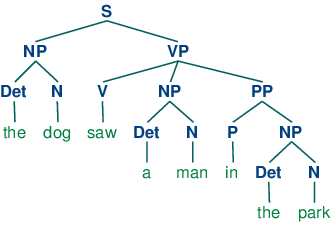
\includegraphics[width=.7\linewidth]{Bilder/grammar_tree.png}
			\caption{Example of a grammar tree. Source: https://www.nltk.org/book/ch08.html}
		\end{figure}
		
		%See also module "23-LIN-Inf Computerlinguistische Grundlagen für Informatik-Studierende"
	\end{frame}
	
	\begin{frame}{Beyong Grammar}
		More intensive forms of analysis can involve:
		\begin{itemize}
			\item[-] Statistical analysis of sentences/phrases
			\item[-] tagging of phrases
			\item[-] dependency parsing
			\item[-] tokenization
		\end{itemize} 
	\end{frame}
	
	\begin{frame}{What do we use?}
		With Pocketsphinx: 
		
		\pause
		Not that much :(
		
		With Google Speechrec:
		
		\pause
		spaCy, a python library which can...
		\begin{itemize}
			\item[-] create a grammar tree of a sentence
			\item[-] classify phrases and words (in context)
			\item[-] abstract information out of text
			\item[-] analyse the similarity of two sentences
		\end{itemize}
	\end{frame}
	
	\begin{frame}{spaCy example}
		From Wikipedia:
		
		\emph{"RoboCup is an annual international robotics competition proposed and founded in 1996 (Pre-RoboCup) by a group of university professors (among which Hiroaki Kitano, Manuela M. Veloso, and Minoru Asada). The aim of such a competition consists of promoting robotics and AI research, by offering a publicly appealing, but formidable challenge."}
		\pause
		
		spaCy:
		
		RoboCup ORG,
		1996 DATE,
		Hiroaki Kitano ORG,
		Manuela M. Veloso PERSON,
		Minoru Asada PERSON,
		AI GPE
	\end{frame}
	
	\begin{frame}{}
		Thanks for the Attention!
	\end{frame}
	
	\begin{frame}{}
		Discussion
	\end{frame}
	
	
	\begin{frame}{Sources}
		\bibliography{demo}
		\bibliographystyle{plain}
	\end{frame}
	
\end{document}
	
	
	
	
	
	
	
	
	
	
	
	
	
	
	
	
	
	
	
	
	%\section{Motivation}%%%%%%%%%%%%%%%%%%%%%%%%%%%%%%%%%%%%%%%%%%%%%%%%%%%%%%%%%%%%%%%%%%%%%
	
	\begin{frame}{Interlude: Hyperparameter I}
		Was sind Hyperparameter?
		\pause
		\begin{itemize}
			\item Werden \emph{vor} dem Lernen definiert
			\item Sind in der Regel Zahlen oder Funktionen
		\end{itemize}
		\pause
		\begin{alertblock}{Allgemein}
			Alles was in irgendeiner Art austauschbar ist in einem speziellen ML-Verfahren und während des Trainings konstant bleibt
		\end{alertblock}
	\end{frame}
	
	\begin{frame}{Interlude: Hyperparameter II}
		Beispiele für Hyperparameter
		\begin{itemize}
			\item Lernrate
			\item (manche) Gewichte
			\item Anzahl der Cluster in k-means clustering
			\item Aktivierungsfunktionen
			\item Anzahl der Hidden Layers in einem Netz
			\item Breite der Layers in einem Netz
		\end{itemize}
	\end{frame}
	
	\begin{frame}{Motivation}
		\begin{itemize}
			\item Einen guten Klassifikator zu trainieren ist schwer, braucht viel Arbeitszeit und Erfahrung
			\item Jeder sollte in der Lage sein Klassifikatoren zu trainieren (im besten Fall sogar Maschinen!)
		\end{itemize}
		\pause
		\alert{Lösung: Ein automatisches (und effizientes) System, welches gute Hyperparameter auswählt, muss her!}
	\end{frame}
	
	
	%\section{Automated Machine Learning in a Nutshell}%%%%%%%%%%%%%%%%%%%%%%%%%%%%%%%%%%%%%%%%%%%%%%%%%%%%%%%%%%%%%%%%%%%%%%%%%%%%%%%%
	
	
	\begin{frame}{Auto-ML I}
		\begin{alertblock}{Grundlegende Idee}
			\begin{itemize}
				\item Classifier trainieren
				\item Classifier evaluieren
				\item Hyperparametertuning mithilfe eines Bayesian optimizer
				\item Wiederholung bis zu einem zufriedenstellenden Ergebnis
				\item Starten mit \emph{irgendwie} ausgewählten Hyperparametern
			\end{itemize}
		\end{alertblock}
	\end{frame}
	
	
	\begin{frame}{Rapidly Exploring Random Tree (RRT) I}
		\begin{alertblock}{Idee}
			\begin{itemize}
				\item Werte zufällig wählen
				\item Punkt im Searchspace analysieren
				\item So oft wiederholen, bis man einen guten Überblick über den Searchspace hat
			\end{itemize}
		\end{alertblock}
		\pause
		\begin{alertblock}{Vorteil}
			Bietet beliebig guten Überblick über den Searchspace
		\end{alertblock}
		\pause
		\begin{alertblock}{Achtung}
			RRT bietet einige Fallstricke. Think before use!
		\end{alertblock}
	\end{frame}
	
	\begin{frame}{Rapidly Exploring Random Tree (RRT) II}
		\centering
		\movie[width=1.0\textwidth,poster,autostart,showcontrols,loop]{
\includegraphics[width=1.0\textwidth]{Bilder/RTT-0.png}}{Bilder/RTT.mp4}
	\end{frame}
	
	\begin{frame}{Probleme bisher}
		\begin{itemize}
			\item Ausgesprochen Rechenintensiv
			\item Unterschiedliche Lernverfahren?
			\item Es gibt kein ``best'' Lernverfahren, nur ``best at''
			\item Manche ML-Verfahren erfordern intensive Hyperparameteroptimisierung
			\item Bayes optimization sollte sich jedoch um dieses Problem kümmern
		\end{itemize}
	\end{frame}
	
	%\section{Meta Learning}%%%%%%%%%%%%%%%%%%%%%%%%%%%%%%%%%%%%%%%%%%%%%%%%%%%%%%%%%%%%%%%%%%%%%%%%%%%%%%%%
	
	\begin{frame}{Meta Learning}
		\begin{alertblock}{Idee}
			\begin{itemize}
				\item Das richtige ML-Verfahren für ein bestimmtes Datenset hängt vom Datenset selbst ab
				\item Ein bestimmter Klassifikator sollte auf ähnlichen Datensets ähnlich gute Ergebnisse liefern
				\pause
			\end{itemize}
			$\Rightarrow$ Also bauen wir uns einen Klassifikator, der uns anhand eines neuen Datensets sagt, welche Art von Klassifikator wir trainieren sollten
		\end{alertblock}
	\end{frame}
	
	\begin{frame}{Im Detail}
		\begin{alertblock}{Erstellung des Meta-Klassifikators}
			\begin{itemize}
				\item Für eine (große) Menge an bereits bekannten Sets: Metafeatures berechnen \\ $\Rightarrow$ class-probability, categorical-numerical-ratio, number of classes/features/instances (missing)
				\item Einen Klassifikator (SMAC) auf diesen Meta-Features trainieren
			\end{itemize}
		\end{alertblock}
		\pause
		\begin{alertblock}{Auswertung}
			\begin{itemize}
				\item Für ein neues Datenset werden anhand der $L_1$ Distanz zu den bereits bekannten Datensets Klassifikatoren ausgewählt
			\end{itemize}
		\end{alertblock}
	\end{frame}
	
	% FORMICA
	% flexible, framework
	% observatory, of
	% robust, robotic 
	% modular
	% interdisziplanary
	% cognitive
	% ants
	
	%\section{Ensembles}%%%%%%%%%%%%%%%%%%%%%%%%%%%%%%%%%%%%%%%%%%%%%%%%%%%%%%%%%%%%%%%%%%%%%%%%%%%%%%%%
	
	\begin{frame}{Bestandsaufnahme}
		\begin{itemize}
			\item Mehrere vielversprechende ML-Verfahren ausgewählt
			\item Jedes davon aufwändig mit Bayesian optimizer im Hinblick auf Hyperparameter getunt
			\item Das beste der Besten herausgepickt und die anderen weggeworfen
		\end{itemize}
		\pause
		\alert{\LARGE{Warum eigentlich?}}
	\end{frame}
	
	\begin{frame}{Ensembles}
		\begin{alertblock}{Idee}
			\begin{itemize}
				\item Anstatt teuer optimierte Klassifikatoren wegzuwerfen, Kombination der Besten
			\end{itemize}
		\end{alertblock}
		\pause
		\alert{Aber wie kombinieren?}
		\begin{itemize}
			\item Alle ungewichtet aufsummieren?
			\item Stacking?
			\item gradient-free numerical optimization?
		\end{itemize}
	\end{frame}
	
	\begin{frame}{Ensemble Selection}
		\begin{alertblock}{Wie baut man ein Ensemble?}
			\begin{itemize}
				\item Starte mit einem leeren Ensemble
				\item Füge den Klassifikator dem Ensemble hinzu, der das Ensemble am besten ergänzt
				\item Wiederhole bis alle Klassifikatoren enthalten sind oder X mal
				\item Durchschnitt über alle Predictions bilden für Resultat
				\pause
				\item Alle Einträge sind ungewichtet
				\item Duplikationen sind erlaubt
			\end{itemize}
	\end{alertblock}
	\end{frame}
	
	
	%\section{Anwendung und Ergebnisse}%%%%%%%%%%%%%%%%%%%%%%%%%%%%%%%%%%%%%%%
	
	\begin{frame}{Anwendung und Evaluation}
		\begin{alertblock}{Setup}
			\begin{itemize}
				\item Meta-learning mit 38 Features für 24h auf 140 OpenML Datensets (2/3 zu 1/3)
				\item Bayesian optimizer auf den 25 besten, Ensemble mit Größe 50
			\end{itemize}
		\end{alertblock}
		\pause
		\begin{alertblock}{Auffälligkeiten und Ergebnisse}
			\begin{itemize}
				\item Meta-learning und Ensemble Selection verbessert bisherige Ansätze deutlich
				\item Besonders bei kurzer Rechenzeit performt die Kombination ML+ES signifikant besser
				\item Mithilfe von ML+ES wird in der Regel ein hinreichend optimaler Klassifikator gefunden
			\end{itemize}
		\end{alertblock}
	\end{frame}
	
	
	\begin{frame}{Recap}
		\begin{alertblock}{Errungenschaften}
			\begin{itemize}
				\item Automatisiertes Maschinenlernen!
				\item Gute Ergebnisse sind auch ohne Vorwissen oder genaue Kenntnisse der einzelnen Verfahren möglich
			\end{itemize}
		\end{alertblock}
		\pause
		\begin{alertblock}{bleibende/ ungelöste Probleme}
			\begin{itemize}
				\item Rechenkosten
				\item Für sehr rechenaufwendige Verfahren (z.b. Deep Learning) nur eingeschränkt zu gebrauchen
				\pause
				\item Wird aber durch recht gute Parallelisierbarkeit teilweise wieder ausgeglichen 
			\end{itemize}
		\end{alertblock}
	\end{frame}
	
	
	\begin{frame}{}
			Vielen Dank für eure Aufmerksamkeit!
	\end{frame}
	
	%\section{Fragerunde}%%%%%%%%%%%%%%%%%%%%%%%%%%%%%%%%%%%%%%%%%%%%%%%%%%%%%%%%%%%%%%%%%%%%%%%%%%%%%%%%%%%%%%%%%
	
	
\end{document}
	
	
	